\documentclass[10pt,a4paper]{article}
\usepackage[margin=19mm]{geometry}
\usepackage[T1]{fontenc}
\usepackage{lmodern,microtype,amsmath,graphicx,booktabs,tabularx,xcolor}
\usepackage[hidelinks,pdfauthor={},pdftitle={Robotics Localization - Technical Brief Report}]{hyperref}
\usepackage{enumitem}
\setlength{\parindent}{0pt}
\setlength{\parskip}{5pt}
\setlist[itemize]{nosep,leftmargin=15pt}
\definecolor{navy}{HTML}{234C69}
\usepackage{titlesec}
\titleformat{\section}{\large\bfseries\color{navy}}{}{0em}{}
\titlespacing*{\section}{0pt}{11pt}{5pt}
\pagestyle{plain}
\begin{document}
{\LARGE\bfseries Robotics localization}\par
{\large\color{navy}Technical Brief Report}\par
\vspace{3pt}
Three course exercises explore how motion models and uncertain observations estimate a robot's position. The implementations cover a position Kalman filter, a five-state Extended Kalman Filter (EKF), and global drone localization with a particle filter. Each algorithm is shared by a ROS 1 node and a reproducible Python simulation.

\section*{Estimation models}
\textbf{Position Kalman filter.} The ground robot travels at a commanded speed of 0.3\,m/s. Its state is planar position $\mathbf p=[x,y]^T$, while measured yaw $\psi$ supplies the displacement input:
\[
\mathbf p^-_t=\mathbf p_{t-1}+v\Delta t
\begin{bmatrix}\cos\psi_t\\\sin\psi_t\end{bmatrix}.
\]
The position-state transition is linear, with identity measurement mapping for GPS. A local input Jacobian maps heading and speed uncertainty into process covariance. GPS, with a 0.3\,m standard deviation in each axis, corrects the prediction. The supplied heading simulator uses the absolute value of Gaussian noise, introducing a positive bias that the replay preserves. This filter does not estimate heading as an independent state.

\textbf{Extended Kalman filter.} The nonlinear state is $[x,y,\theta,v,\omega]^T$. Exact constant-turn-rate integration predicts circular motion at nominal values $v=0.5$\,m/s and $\omega=0.3$\,rad/s. Written with midpoint angle $\phi=\theta+\omega\Delta t/2$, the displacement is
\[
\Delta\mathbf p=v\Delta t\,\operatorname{sinc}(\omega\Delta t/2)
\begin{bmatrix}\cos\phi\\\sin\phi\end{bmatrix},\qquad
\operatorname{sinc}(u)=\frac{\sin u}{u}.
\]
A small-angle series preserves the zero-turn limit. An analytic Jacobian propagates covariance. Position and velocity observations then correct the five-state estimate. The provided GPS generator shares one noise sample between axes, so its default covariance models that correlation rather than treating the coordinates as independent.

\textbf{Particle filter.} A uniform prior distributes 12,000 particles across an 8\,$\times$\,15\,m grid. Noisy displacements move particles, and the height-map likelihood compares each proposed surface height with altitude minus downward range. Log-space weights avoid underflow. Effective sample size $N_\mathrm{eff}=1/\sum_i w_i^2$ triggers systematic resampling below $N/2$. Invalid positions are replaced inside the domain. The ROS output is a \texttt{PoseArray} in frame \texttt{map}, with particle height 1\,m and identity orientation.

\begin{center}
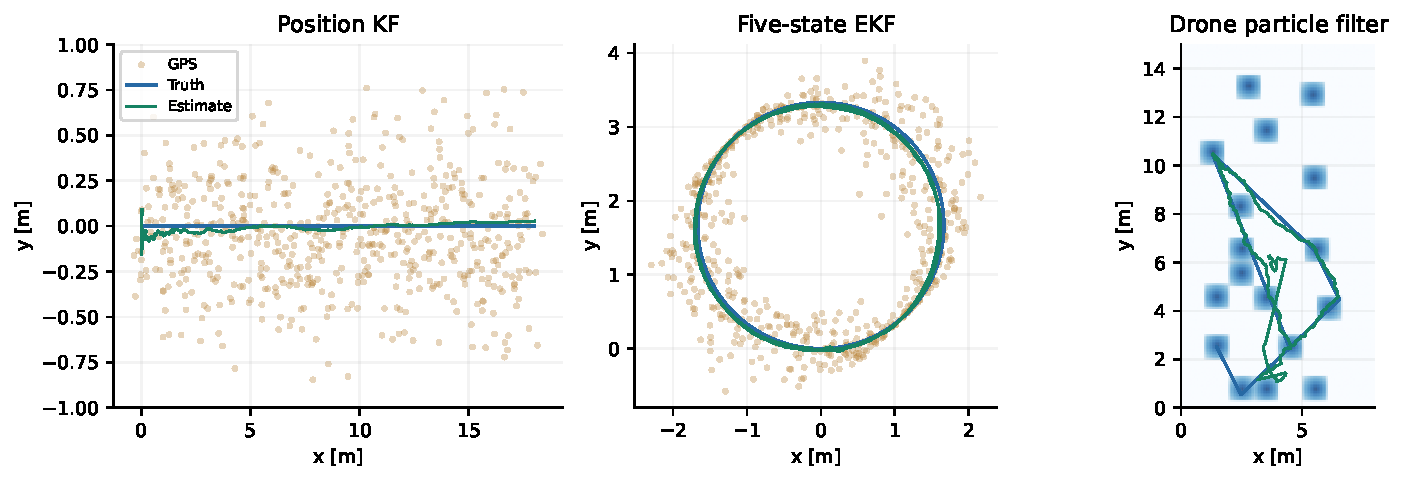
\includegraphics[width=\linewidth]{assets/trajectories.pdf}
\end{center}
\vspace{-5pt}
{\small\textbf{Simulation trajectories.} Blue denotes true position and green the estimate. The first two panels include noisy GPS. The drone panel uses the supplied world's encoded measurement surface. The initial particle mean can lie between distinct position hypotheses.}

\newpage
\section*{Implementation and integration}
All numerical cores depend only on NumPy. ROS imports are deferred or optional, allowing the same source files to run without a ROS installation. Kalman updates use linear solves rather than explicit matrix inversion and Joseph-form covariance updates. Heading is wrapped after EKF prediction and correction.

The position node advances on timestamped GPS callbacks and publishes the latest result at 10\,Hz. The EKF adapter fuses each latest GPS and velocity sample once at a 10\,Hz tick, rejecting samples older than 0.5\,s. This is approximate asynchronous fusion, not retrospective smoothing. The particle node obtains observations exclusively through the three supplied measurement helpers, whose bodies are unchanged.

The offline drone map uses saved SDF state poses, which override different model-definition poses in the archived world. A test compares the resulting grid directly with the provided map-building helper on the same model states. The scalar height profile follows the exercise's decreasing values around box centers, rather than flat physical box tops.

\section*{Reproducible results}
All reported values use seed 7 and a 0.1\,s step. Ground-robot noise follows the supplied sensor generators. Drone measurements use independent uniform errors of $\pm0.05$\,m. The drone route is prescribed for this synthetic experiment. Two-dimensional position RMSE is $\sqrt{\frac1T\sum_t\|\hat{\mathbf p}_t-\mathbf p_t\|^2}$.

\begin{center}
\begin{tabular}{@{}lrrr@{}}
\toprule
Replay & Duration & GPS RMSE & Estimate RMSE\\
\midrule
Position KF & 60.0\,s & 0.406\,m & 0.049\,m\\
Five-state EKF & 63.0\,s & 0.331\,m & 0.063\,m\\
\bottomrule
\end{tabular}
\end{center}
The particle replay runs for 35.4\,s (355 samples). Its initial weighted-mean error is 4.353\,m and final error is 0.045\,m. RMSE over the final 100 samples is 0.195\,m. Initial global ambiguity makes the early weighted mean a poor summary of a multimodal posterior. These values describe one seeded route and do not establish convergence for every route or noise realization.

\section*{Validation and scope}
Ten automated tests cover an independent closed-form KF posterior, straight-line prediction, invalid input, numerical checks of the EKF Jacobian, analytic circles, the zero-turn limit, covariance symmetry and positivity, particle bounds and resampling, map-helper equivalence, and all three replay scenarios. The browser capture tool additionally checks that playback controls change the rendered canvas before saving screenshots.

The verified execution is Python simulation on Linux. The browser visualizes stored algorithm output and does not implement alternative filters. ROS, RViz, Gazebo dynamics, external robot packages, and physical hardware were not exercised. The provided sensor helpers use simulation-derived pose information. Their blocking calls and timing behavior are not replicated by the offline replay. Neither statistical calibration of covariance contours nor real-time performance is established by the current checks.

\section*{Run and inspect}
\begin{verbatim}
python3 -m pip install -r requirements.txt
python3 -m unittest discover -s tests -v
python3 tools/simulate.py
python3 -m http.server 8765 --bind 127.0.0.1
\end{verbatim}
Open \texttt{http://127.0.0.1:8765/tools/viewer.html}. Each assignment directory contains its own README, implementation, ROS package, and links to the corresponding screenshot. \href{https://github.com/mitsosasim/robotics_uoc/blob/main/docs/SETUP.md}{The setup guide} documents dependencies, external model paths, and ROS commands. Course scaffolding and world data originate in the CS-475 materials by Michael Maravgakis. The current filter implementations are reconstructed course exercises.
\end{document}
